% Created by tikzDevice version 0.12
% !TEX encoding = UTF-8 Unicode
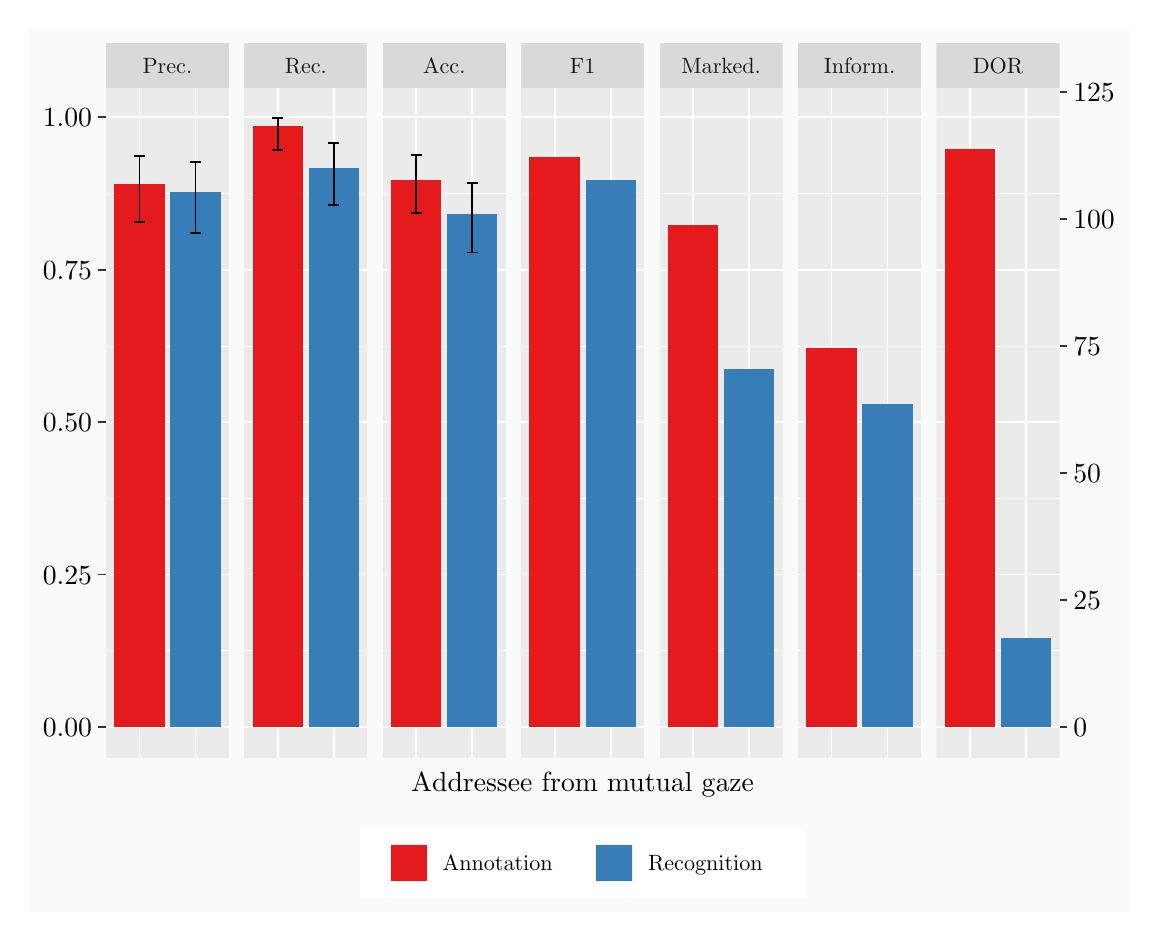
\begin{tikzpicture}[x=1pt,y=1pt]
\definecolor{fillColor}{RGB}{255,255,255}
\path[use as bounding box,fill=fillColor,fill opacity=0.00] (0,0) rectangle (398.34,320.03);
\begin{scope}
\path[clip] (  0.00,  0.00) rectangle (398.34,320.03);
\definecolor{drawColor}{RGB}{255,255,255}
\definecolor{fillColor}{gray}{0.98}

\path[draw=drawColor,line width= 0.6pt,line join=round,line cap=round,fill=fillColor] (  0.00,  0.00) rectangle (398.34,320.03);
\end{scope}
\begin{scope}
\path[clip] ( 28.22, 56.29) rectangle ( 72.75,298.27);
\definecolor{fillColor}{gray}{0.92}

\path[fill=fillColor] ( 28.22, 56.29) rectangle ( 72.75,298.27);
\definecolor{drawColor}{RGB}{255,255,255}

\path[draw=drawColor,line width= 0.3pt,line join=round] ( 28.22, 94.83) --
	( 72.75, 94.83);

\path[draw=drawColor,line width= 0.3pt,line join=round] ( 28.22,149.93) --
	( 72.75,149.93);

\path[draw=drawColor,line width= 0.3pt,line join=round] ( 28.22,205.03) --
	( 72.75,205.03);

\path[draw=drawColor,line width= 0.3pt,line join=round] ( 28.22,260.13) --
	( 72.75,260.13);

\path[draw=drawColor,line width= 0.6pt,line join=round] ( 28.22, 67.28) --
	( 72.75, 67.28);

\path[draw=drawColor,line width= 0.6pt,line join=round] ( 28.22,122.38) --
	( 72.75,122.38);

\path[draw=drawColor,line width= 0.6pt,line join=round] ( 28.22,177.48) --
	( 72.75,177.48);

\path[draw=drawColor,line width= 0.6pt,line join=round] ( 28.22,232.58) --
	( 72.75,232.58);

\path[draw=drawColor,line width= 0.6pt,line join=round] ( 28.22,287.68) --
	( 72.75,287.68);

\path[draw=drawColor,line width= 0.6pt,line join=round] ( 40.37, 56.29) --
	( 40.37,298.27);

\path[draw=drawColor,line width= 0.6pt,line join=round] ( 60.60, 56.29) --
	( 60.60,298.27);
\definecolor{fillColor}{RGB}{228,26,28}

\path[fill=fillColor] ( 31.26, 67.28) rectangle ( 49.47,263.53);
\definecolor{fillColor}{RGB}{55,126,184}

\path[fill=fillColor] ( 51.50, 67.28) rectangle ( 69.71,260.53);
\definecolor{drawColor}{RGB}{0,0,0}

\path[draw=drawColor,line width= 0.6pt,line join=round] ( 58.58,271.49) --
	( 62.63,271.49);

\path[draw=drawColor,line width= 0.6pt,line join=round] ( 60.60,271.49) --
	( 60.60,245.83);

\path[draw=drawColor,line width= 0.6pt,line join=round] ( 58.58,245.83) --
	( 62.63,245.83);

\path[draw=drawColor,line width= 0.6pt,line join=round] ( 38.34,273.58) --
	( 42.39,273.58);

\path[draw=drawColor,line width= 0.6pt,line join=round] ( 40.37,273.58) --
	( 40.37,249.80);

\path[draw=drawColor,line width= 0.6pt,line join=round] ( 38.34,249.80) --
	( 42.39,249.80);
\end{scope}
\begin{scope}
\path[clip] ( 78.25, 56.29) rectangle (122.77,298.27);
\definecolor{fillColor}{gray}{0.92}

\path[fill=fillColor] ( 78.25, 56.29) rectangle (122.77,298.27);
\definecolor{drawColor}{RGB}{255,255,255}

\path[draw=drawColor,line width= 0.3pt,line join=round] ( 78.25, 94.83) --
	(122.77, 94.83);

\path[draw=drawColor,line width= 0.3pt,line join=round] ( 78.25,149.93) --
	(122.77,149.93);

\path[draw=drawColor,line width= 0.3pt,line join=round] ( 78.25,205.03) --
	(122.77,205.03);

\path[draw=drawColor,line width= 0.3pt,line join=round] ( 78.25,260.13) --
	(122.77,260.13);

\path[draw=drawColor,line width= 0.6pt,line join=round] ( 78.25, 67.28) --
	(122.77, 67.28);

\path[draw=drawColor,line width= 0.6pt,line join=round] ( 78.25,122.38) --
	(122.77,122.38);

\path[draw=drawColor,line width= 0.6pt,line join=round] ( 78.25,177.48) --
	(122.77,177.48);

\path[draw=drawColor,line width= 0.6pt,line join=round] ( 78.25,232.58) --
	(122.77,232.58);

\path[draw=drawColor,line width= 0.6pt,line join=round] ( 78.25,287.68) --
	(122.77,287.68);

\path[draw=drawColor,line width= 0.6pt,line join=round] ( 90.39, 56.29) --
	( 90.39,298.27);

\path[draw=drawColor,line width= 0.6pt,line join=round] (110.63, 56.29) --
	(110.63,298.27);
\definecolor{fillColor}{RGB}{228,26,28}

\path[fill=fillColor] ( 81.28, 67.28) rectangle ( 99.50,284.34);
\definecolor{fillColor}{RGB}{55,126,184}

\path[fill=fillColor] (101.52, 67.28) rectangle (119.74,269.31);
\definecolor{drawColor}{RGB}{0,0,0}

\path[draw=drawColor,line width= 0.6pt,line join=round] (108.60,278.35) --
	(112.65,278.35);

\path[draw=drawColor,line width= 0.6pt,line join=round] (110.63,278.35) --
	(110.63,255.89);

\path[draw=drawColor,line width= 0.6pt,line join=round] (108.60,255.89) --
	(112.65,255.89);

\path[draw=drawColor,line width= 0.6pt,line join=round] ( 88.37,287.27) --
	( 92.41,287.27);

\path[draw=drawColor,line width= 0.6pt,line join=round] ( 90.39,287.27) --
	( 90.39,275.85);

\path[draw=drawColor,line width= 0.6pt,line join=round] ( 88.37,275.85) --
	( 92.41,275.85);
\end{scope}
\begin{scope}
\path[clip] (128.27, 56.29) rectangle (172.80,298.27);
\definecolor{fillColor}{gray}{0.92}

\path[fill=fillColor] (128.27, 56.29) rectangle (172.80,298.27);
\definecolor{drawColor}{RGB}{255,255,255}

\path[draw=drawColor,line width= 0.3pt,line join=round] (128.27, 94.83) --
	(172.80, 94.83);

\path[draw=drawColor,line width= 0.3pt,line join=round] (128.27,149.93) --
	(172.80,149.93);

\path[draw=drawColor,line width= 0.3pt,line join=round] (128.27,205.03) --
	(172.80,205.03);

\path[draw=drawColor,line width= 0.3pt,line join=round] (128.27,260.13) --
	(172.80,260.13);

\path[draw=drawColor,line width= 0.6pt,line join=round] (128.27, 67.28) --
	(172.80, 67.28);

\path[draw=drawColor,line width= 0.6pt,line join=round] (128.27,122.38) --
	(172.80,122.38);

\path[draw=drawColor,line width= 0.6pt,line join=round] (128.27,177.48) --
	(172.80,177.48);

\path[draw=drawColor,line width= 0.6pt,line join=round] (128.27,232.58) --
	(172.80,232.58);

\path[draw=drawColor,line width= 0.6pt,line join=round] (128.27,287.68) --
	(172.80,287.68);

\path[draw=drawColor,line width= 0.6pt,line join=round] (140.41, 56.29) --
	(140.41,298.27);

\path[draw=drawColor,line width= 0.6pt,line join=round] (160.65, 56.29) --
	(160.65,298.27);
\definecolor{fillColor}{RGB}{228,26,28}

\path[fill=fillColor] (131.31, 67.28) rectangle (149.52,265.14);
\definecolor{fillColor}{RGB}{55,126,184}

\path[fill=fillColor] (151.55, 67.28) rectangle (169.76,252.62);
\definecolor{drawColor}{RGB}{0,0,0}

\path[draw=drawColor,line width= 0.6pt,line join=round] (158.63,263.79) --
	(162.68,263.79);

\path[draw=drawColor,line width= 0.6pt,line join=round] (160.65,263.79) --
	(160.65,238.83);

\path[draw=drawColor,line width= 0.6pt,line join=round] (158.63,238.83) --
	(162.68,238.83);

\path[draw=drawColor,line width= 0.6pt,line join=round] (138.39,274.07) --
	(142.44,274.07);

\path[draw=drawColor,line width= 0.6pt,line join=round] (140.41,274.07) --
	(140.41,253.12);

\path[draw=drawColor,line width= 0.6pt,line join=round] (138.39,253.12) --
	(142.44,253.12);
\end{scope}
\begin{scope}
\path[clip] (178.30, 56.29) rectangle (222.82,298.27);
\definecolor{fillColor}{gray}{0.92}

\path[fill=fillColor] (178.30, 56.29) rectangle (222.82,298.27);
\definecolor{drawColor}{RGB}{255,255,255}

\path[draw=drawColor,line width= 0.3pt,line join=round] (178.30, 94.83) --
	(222.82, 94.83);

\path[draw=drawColor,line width= 0.3pt,line join=round] (178.30,149.93) --
	(222.82,149.93);

\path[draw=drawColor,line width= 0.3pt,line join=round] (178.30,205.03) --
	(222.82,205.03);

\path[draw=drawColor,line width= 0.3pt,line join=round] (178.30,260.13) --
	(222.82,260.13);

\path[draw=drawColor,line width= 0.6pt,line join=round] (178.30, 67.28) --
	(222.82, 67.28);

\path[draw=drawColor,line width= 0.6pt,line join=round] (178.30,122.38) --
	(222.82,122.38);

\path[draw=drawColor,line width= 0.6pt,line join=round] (178.30,177.48) --
	(222.82,177.48);

\path[draw=drawColor,line width= 0.6pt,line join=round] (178.30,232.58) --
	(222.82,232.58);

\path[draw=drawColor,line width= 0.6pt,line join=round] (178.30,287.68) --
	(222.82,287.68);

\path[draw=drawColor,line width= 0.6pt,line join=round] (190.44, 56.29) --
	(190.44,298.27);

\path[draw=drawColor,line width= 0.6pt,line join=round] (210.68, 56.29) --
	(210.68,298.27);
\definecolor{fillColor}{RGB}{228,26,28}

\path[fill=fillColor] (181.33, 67.28) rectangle (199.55,273.41);
\definecolor{fillColor}{RGB}{55,126,184}

\path[fill=fillColor] (201.57, 67.28) rectangle (219.78,264.82);
\end{scope}
\begin{scope}
\path[clip] (228.32, 56.29) rectangle (272.84,298.27);
\definecolor{fillColor}{gray}{0.92}

\path[fill=fillColor] (228.32, 56.29) rectangle (272.84,298.27);
\definecolor{drawColor}{RGB}{255,255,255}

\path[draw=drawColor,line width= 0.3pt,line join=round] (228.32, 94.83) --
	(272.84, 94.83);

\path[draw=drawColor,line width= 0.3pt,line join=round] (228.32,149.93) --
	(272.84,149.93);

\path[draw=drawColor,line width= 0.3pt,line join=round] (228.32,205.03) --
	(272.84,205.03);

\path[draw=drawColor,line width= 0.3pt,line join=round] (228.32,260.13) --
	(272.84,260.13);

\path[draw=drawColor,line width= 0.6pt,line join=round] (228.32, 67.28) --
	(272.84, 67.28);

\path[draw=drawColor,line width= 0.6pt,line join=round] (228.32,122.38) --
	(272.84,122.38);

\path[draw=drawColor,line width= 0.6pt,line join=round] (228.32,177.48) --
	(272.84,177.48);

\path[draw=drawColor,line width= 0.6pt,line join=round] (228.32,232.58) --
	(272.84,232.58);

\path[draw=drawColor,line width= 0.6pt,line join=round] (228.32,287.68) --
	(272.84,287.68);

\path[draw=drawColor,line width= 0.6pt,line join=round] (240.46, 56.29) --
	(240.46,298.27);

\path[draw=drawColor,line width= 0.6pt,line join=round] (260.70, 56.29) --
	(260.70,298.27);
\definecolor{fillColor}{RGB}{228,26,28}

\path[fill=fillColor] (231.36, 67.28) rectangle (249.57,248.83);
\definecolor{fillColor}{RGB}{55,126,184}

\path[fill=fillColor] (251.59, 67.28) rectangle (269.81,196.73);
\end{scope}
\begin{scope}
\path[clip] (278.34, 56.29) rectangle (322.87,298.27);
\definecolor{fillColor}{gray}{0.92}

\path[fill=fillColor] (278.34, 56.29) rectangle (322.87,298.27);
\definecolor{drawColor}{RGB}{255,255,255}

\path[draw=drawColor,line width= 0.3pt,line join=round] (278.34, 94.83) --
	(322.87, 94.83);

\path[draw=drawColor,line width= 0.3pt,line join=round] (278.34,149.93) --
	(322.87,149.93);

\path[draw=drawColor,line width= 0.3pt,line join=round] (278.34,205.03) --
	(322.87,205.03);

\path[draw=drawColor,line width= 0.3pt,line join=round] (278.34,260.13) --
	(322.87,260.13);

\path[draw=drawColor,line width= 0.6pt,line join=round] (278.34, 67.28) --
	(322.87, 67.28);

\path[draw=drawColor,line width= 0.6pt,line join=round] (278.34,122.38) --
	(322.87,122.38);

\path[draw=drawColor,line width= 0.6pt,line join=round] (278.34,177.48) --
	(322.87,177.48);

\path[draw=drawColor,line width= 0.6pt,line join=round] (278.34,232.58) --
	(322.87,232.58);

\path[draw=drawColor,line width= 0.6pt,line join=round] (278.34,287.68) --
	(322.87,287.68);

\path[draw=drawColor,line width= 0.6pt,line join=round] (290.49, 56.29) --
	(290.49,298.27);

\path[draw=drawColor,line width= 0.6pt,line join=round] (310.73, 56.29) --
	(310.73,298.27);
\definecolor{fillColor}{RGB}{228,26,28}

\path[fill=fillColor] (281.38, 67.28) rectangle (299.59,204.20);
\definecolor{fillColor}{RGB}{55,126,184}

\path[fill=fillColor] (301.62, 67.28) rectangle (319.83,184.16);
\end{scope}
\begin{scope}
\path[clip] (328.37, 56.29) rectangle (372.89,298.27);
\definecolor{fillColor}{gray}{0.92}

\path[fill=fillColor] (328.37, 56.29) rectangle (372.89,298.27);
\definecolor{drawColor}{RGB}{255,255,255}

\path[draw=drawColor,line width= 0.3pt,line join=round] (328.37, 94.83) --
	(372.89, 94.83);

\path[draw=drawColor,line width= 0.3pt,line join=round] (328.37,149.93) --
	(372.89,149.93);

\path[draw=drawColor,line width= 0.3pt,line join=round] (328.37,205.03) --
	(372.89,205.03);

\path[draw=drawColor,line width= 0.3pt,line join=round] (328.37,260.13) --
	(372.89,260.13);

\path[draw=drawColor,line width= 0.6pt,line join=round] (328.37, 67.28) --
	(372.89, 67.28);

\path[draw=drawColor,line width= 0.6pt,line join=round] (328.37,122.38) --
	(372.89,122.38);

\path[draw=drawColor,line width= 0.6pt,line join=round] (328.37,177.48) --
	(372.89,177.48);

\path[draw=drawColor,line width= 0.6pt,line join=round] (328.37,232.58) --
	(372.89,232.58);

\path[draw=drawColor,line width= 0.6pt,line join=round] (328.37,287.68) --
	(372.89,287.68);

\path[draw=drawColor,line width= 0.6pt,line join=round] (340.51, 56.29) --
	(340.51,298.27);

\path[draw=drawColor,line width= 0.6pt,line join=round] (360.75, 56.29) --
	(360.75,298.27);
\definecolor{fillColor}{RGB}{228,26,28}

\path[fill=fillColor] (331.40, 67.28) rectangle (349.62,276.20);
\definecolor{fillColor}{RGB}{55,126,184}

\path[fill=fillColor] (351.64, 67.28) rectangle (369.86, 99.37);
\end{scope}
\begin{scope}
\path[clip] ( 28.22,298.27) rectangle ( 72.75,314.53);
\definecolor{fillColor}{gray}{0.85}

\path[fill=fillColor] ( 28.22,298.27) rectangle ( 72.75,314.53);
\definecolor{drawColor}{gray}{0.10}

\node[text=drawColor,anchor=base,inner sep=0pt, outer sep=0pt, scale=  0.80] at ( 50.49,303.64) {Prec.};
\end{scope}
\begin{scope}
\path[clip] ( 78.25,298.27) rectangle (122.77,314.53);
\definecolor{fillColor}{gray}{0.85}

\path[fill=fillColor] ( 78.25,298.27) rectangle (122.77,314.53);
\definecolor{drawColor}{gray}{0.10}

\node[text=drawColor,anchor=base,inner sep=0pt, outer sep=0pt, scale=  0.80] at (100.51,303.64) {Rec.};
\end{scope}
\begin{scope}
\path[clip] (128.27,298.27) rectangle (172.80,314.53);
\definecolor{fillColor}{gray}{0.85}

\path[fill=fillColor] (128.27,298.27) rectangle (172.80,314.53);
\definecolor{drawColor}{gray}{0.10}

\node[text=drawColor,anchor=base,inner sep=0pt, outer sep=0pt, scale=  0.80] at (150.53,303.64) {Acc.};
\end{scope}
\begin{scope}
\path[clip] (178.30,298.27) rectangle (222.82,314.53);
\definecolor{fillColor}{gray}{0.85}

\path[fill=fillColor] (178.30,298.27) rectangle (222.82,314.53);
\definecolor{drawColor}{gray}{0.10}

\node[text=drawColor,anchor=base,inner sep=0pt, outer sep=0pt, scale=  0.80] at (200.56,303.64) {F1};
\end{scope}
\begin{scope}
\path[clip] (228.32,298.27) rectangle (272.84,314.53);
\definecolor{fillColor}{gray}{0.85}

\path[fill=fillColor] (228.32,298.27) rectangle (272.84,314.53);
\definecolor{drawColor}{gray}{0.10}

\node[text=drawColor,anchor=base,inner sep=0pt, outer sep=0pt, scale=  0.80] at (250.58,303.64) {Marked.};
\end{scope}
\begin{scope}
\path[clip] (278.34,298.27) rectangle (322.87,314.53);
\definecolor{fillColor}{gray}{0.85}

\path[fill=fillColor] (278.34,298.27) rectangle (322.87,314.53);
\definecolor{drawColor}{gray}{0.10}

\node[text=drawColor,anchor=base,inner sep=0pt, outer sep=0pt, scale=  0.80] at (300.61,303.64) {Inform.};
\end{scope}
\begin{scope}
\path[clip] (328.37,298.27) rectangle (372.89,314.53);
\definecolor{fillColor}{gray}{0.85}

\path[fill=fillColor] (328.37,298.27) rectangle (372.89,314.53);
\definecolor{drawColor}{gray}{0.10}

\node[text=drawColor,anchor=base,inner sep=0pt, outer sep=0pt, scale=  0.80] at (350.63,303.64) {DOR};
\end{scope}
\begin{scope}
\path[clip] (  0.00,  0.00) rectangle (398.34,320.03);
\definecolor{drawColor}{RGB}{0,0,0}

\node[text=drawColor,anchor=base east,inner sep=0pt, outer sep=0pt, scale=  1.00] at ( 23.27, 63.84) {0.00};

\node[text=drawColor,anchor=base east,inner sep=0pt, outer sep=0pt, scale=  1.00] at ( 23.27,118.94) {0.25};

\node[text=drawColor,anchor=base east,inner sep=0pt, outer sep=0pt, scale=  1.00] at ( 23.27,174.04) {0.50};

\node[text=drawColor,anchor=base east,inner sep=0pt, outer sep=0pt, scale=  1.00] at ( 23.27,229.14) {0.75};

\node[text=drawColor,anchor=base east,inner sep=0pt, outer sep=0pt, scale=  1.00] at ( 23.27,284.23) {1.00};
\end{scope}
\begin{scope}
\path[clip] (  0.00,  0.00) rectangle (398.34,320.03);
\definecolor{drawColor}{gray}{0.20}

\path[draw=drawColor,line width= 0.6pt,line join=round] ( 25.47, 67.28) --
	( 28.22, 67.28);

\path[draw=drawColor,line width= 0.6pt,line join=round] ( 25.47,122.38) --
	( 28.22,122.38);

\path[draw=drawColor,line width= 0.6pt,line join=round] ( 25.47,177.48) --
	( 28.22,177.48);

\path[draw=drawColor,line width= 0.6pt,line join=round] ( 25.47,232.58) --
	( 28.22,232.58);

\path[draw=drawColor,line width= 0.6pt,line join=round] ( 25.47,287.68) --
	( 28.22,287.68);
\end{scope}
\begin{scope}
\path[clip] (  0.00,  0.00) rectangle (398.34,320.03);
\definecolor{drawColor}{gray}{0.20}

\path[draw=drawColor,line width= 0.6pt,line join=round] (372.89, 67.28) --
	(375.64, 67.28);

\path[draw=drawColor,line width= 0.6pt,line join=round] (372.89,113.20) --
	(375.64,113.20);

\path[draw=drawColor,line width= 0.6pt,line join=round] (372.89,159.12) --
	(375.64,159.12);

\path[draw=drawColor,line width= 0.6pt,line join=round] (372.89,205.03) --
	(375.64,205.03);

\path[draw=drawColor,line width= 0.6pt,line join=round] (372.89,250.95) --
	(375.64,250.95);

\path[draw=drawColor,line width= 0.6pt,line join=round] (372.89,296.86) --
	(375.64,296.86);
\end{scope}
\begin{scope}
\path[clip] (  0.00,  0.00) rectangle (398.34,320.03);
\definecolor{drawColor}{RGB}{0,0,0}

\node[text=drawColor,anchor=base west,inner sep=0pt, outer sep=0pt, scale=  1.00] at (377.84, 63.84) {0};

\node[text=drawColor,anchor=base west,inner sep=0pt, outer sep=0pt, scale=  1.00] at (377.84,109.76) {25};

\node[text=drawColor,anchor=base west,inner sep=0pt, outer sep=0pt, scale=  1.00] at (377.84,155.67) {50};

\node[text=drawColor,anchor=base west,inner sep=0pt, outer sep=0pt, scale=  1.00] at (377.84,201.59) {75};

\node[text=drawColor,anchor=base west,inner sep=0pt, outer sep=0pt, scale=  1.00] at (377.84,247.50) {100};

\node[text=drawColor,anchor=base west,inner sep=0pt, outer sep=0pt, scale=  1.00] at (377.84,293.42) {125};
\end{scope}
\begin{scope}
\path[clip] (  0.00,  0.00) rectangle (398.34,320.03);
\definecolor{drawColor}{RGB}{0,0,0}

\node[text=drawColor,anchor=base,inner sep=0pt, outer sep=0pt, scale=  1.00] at (200.56, 43.90) {Addressee from mutual gaze};
\end{scope}
\begin{scope}
\path[clip] (  0.00,  0.00) rectangle (398.34,320.03);
\definecolor{fillColor}{RGB}{255,255,255}

\path[fill=fillColor] (120.00,  5.50) rectangle (281.11, 30.95);
\end{scope}
\begin{scope}
\path[clip] (  0.00,  0.00) rectangle (398.34,320.03);
\definecolor{drawColor}{RGB}{255,255,255}
\definecolor{fillColor}{gray}{0.95}

\path[draw=drawColor,line width= 0.6pt,line join=round,line cap=round,fill=fillColor] (130.50, 11.00) rectangle (144.96, 25.45);
\end{scope}
\begin{scope}
\path[clip] (  0.00,  0.00) rectangle (398.34,320.03);
\definecolor{fillColor}{RGB}{228,26,28}

\path[fill=fillColor] (131.21, 11.71) rectangle (144.25, 24.74);
\end{scope}
\begin{scope}
\path[clip] (  0.00,  0.00) rectangle (398.34,320.03);
\definecolor{drawColor}{RGB}{255,255,255}
\definecolor{fillColor}{gray}{0.95}

\path[draw=drawColor,line width= 0.6pt,line join=round,line cap=round,fill=fillColor] (204.72, 11.00) rectangle (219.18, 25.45);
\end{scope}
\begin{scope}
\path[clip] (  0.00,  0.00) rectangle (398.34,320.03);
\definecolor{fillColor}{RGB}{55,126,184}

\path[fill=fillColor] (205.44, 11.71) rectangle (218.47, 24.74);
\end{scope}
\begin{scope}
\path[clip] (  0.00,  0.00) rectangle (398.34,320.03);
\definecolor{drawColor}{RGB}{0,0,0}

\node[text=drawColor,anchor=base west,inner sep=0pt, outer sep=0pt, scale=  0.80] at (149.96, 15.47) {Annotation};
\end{scope}
\begin{scope}
\path[clip] (  0.00,  0.00) rectangle (398.34,320.03);
\definecolor{drawColor}{RGB}{0,0,0}

\node[text=drawColor,anchor=base west,inner sep=0pt, outer sep=0pt, scale=  0.80] at (224.18, 15.47) {Recognition};
\end{scope}
\end{tikzpicture}
